\chapter{Numerical experiments}
\label{chap:expe}

From the point of view of computational cost, it is convenient to make a brief analysis of the relevant new continuous-time framework obtained in Eq. \ref{eqn:u3.3}. The main problem that we can find when dealing with large networks (matrices) resides in the computation of the matrix logarithm, which can be computationally expensive.

This function computes the natural logarithm of a matrix, which is defined as follows \cite{higham2008functions}:

\begin{definition}
    A logarithm of $A \in \mathbb{C}^{N\times N}$ is any matrix $X$ such that $e^X = A$ where $e^X = I + X + \frac{X^2}{2!} + \frac{X^3}{3!} + \cdots$. If $A$ is assumed to have no eigenvalues on $\mathbb{R}^{-}$, then we call this logarithm to be the principal logarithm of $A$, which is the unique logarithm whose spectrum lies in the strip $\{ z : −\pi < Im(z) < \pi \}$.
\end{definition}

In Python, the \texttt{scipy.linalg.logm} module from the SciPy library computes the logarithm of a matrix using the Schur decomposition with a computational cost of $\mathcal{O}(N^3)$ for an $N \times N$ matrix. However, the Schur decomposition is not always the most efficient way to compute the matrix logarithm, especially for large matrices with special properties such as sparsity or symmetry. In these cases, specialized algorithms may be used to approximate the matrix logarithm reducing its computational cost.

Next, we consider the two synthetic experiments from \cite{grindrod2014dynamical} in order to demonstrate how our new matrix ODE approach works and provide a better understanding of the $\alpha,\beta$ parameters. With this two artificial networks that evolve continuously over time, we intend to show a hierarchy of influence for the nodes that would not be evident if we only considered a static picture or a summarized view of the network. The relatively small size of these examples, 31 and 17 nodes respectively, will facilitate the process of visualizing, and it will also allow us to employ a highly precise Runge-Kutta iteration to solve the corresponding ODE systems (\ref{eqn:u3.3}) with accuracy.

\section{Synthetic experiments}
\label{sec:synexp}
The first synthetic experiment models a cascade of information through the directed binary
tree structure illustrated in Figure \ref{fig:exp1}. On a time interval $t = [0, 20]$, the adjacency
matrix $\mathbf{A}(t)$ of such network switches between two constant values $\mathbf{A}_{even}$ and $\mathbf{A}_{odd}$ on each sub-interval $[i, i + 1)$, specifically

\begin{equation*}
\mathbf{A}(t)=
    \begin{cases}
        \mathbf{A}_{even}, & \text{if } mod(\lfloor t \rfloor, 2) = 0\\
        \mathbf{A}_{odd}, & \text{otherwise} 
    \end{cases}
\end{equation*}

where $\mathbf{A}_{even}$ is the adjacency matrix relative to the subgraph with solid edges in Figure \ref{fig:exp1}, and $\mathbf{A}_{odd}$ the one relative to the subgraph with dashed edges. Some noise to this structure is added by including extra directed edges that are chosen uniformly at random for each subinterval, with an average of five edges added each time. 

This type of structure allows us to clearly visualize the follow-on effect arising from the time-ordering of the interactions.

\begin{figure}[h]\centering
    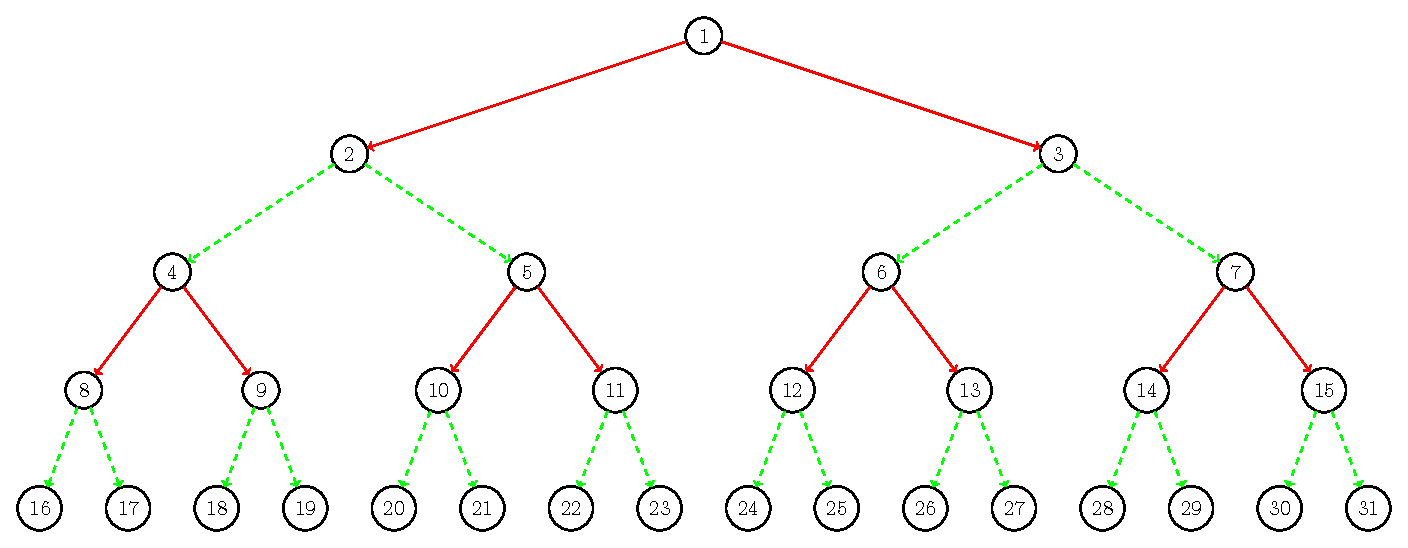
\includegraphics[width=.75\textwidth]{experiment1}
    \caption{Network structure (binary tree) for the first synthetic experiment. The active links of A(t) alternate between the solid and dashed edges, with extra noise added at each time step, over a period of 10 cycles.}
    \label{fig:exp1}
    \bigskip
\end{figure}

Due to the hierarchy and timing of the edges, information appears to flow from lower indices to higher. The binary structure of the tree makes node 1 to be particularly efficient at transmitting information through the network, although this may not be immediately apparent in a single snapshot.

Figure \ref{fig:bt1} displays the dynamic broadcast centrality from Eq. \ref{eqn:u3.4}, at time $t=20$ for each of the 31 nodes. We observe that node 1 has a strong advantage in terms of centrality, and that centrality tends to decrease as the index increases. Nodes 2 and 5 are ranked higher than node 3, indicating that the additional noise has affected this part of the network. Since the maximum spectral radius of $\mathbf{A}(t)$ over the interval $[0, 20]$ is one, the parameter $\alpha=0.7$ was chosen with $\beta=0.1$, in this case.

Figure \ref{fig:bt2} depicts the same results with a lower $\beta=0.01$ value, which increases the contribution of older walks. As a reminder, if we consider a walk starting at time zero, then the  downweighting factor becomes $e^{−20 \times 0.01} \approx 0.8$ rather than $e^{−20 \times 0.1} \approx 0.1$. This change of the $\beta$ parameter has a negligible effect on the node rankings which makes sense considering that the network dynamics have an underlying periodic pattern, but it can be observed that it generates larger absolute values.

In Figure \ref{fig:bt3}, we return to the original $\beta=0.1$ value and set $\alpha$ to 0.1, resulting in less marked differences in the node rankings. Even though node 1 continues to be the most central, the differences are less pronounced as its capability to initiate numerous dynamic walks of length 4 to nodes at the bottom of the hierarchy has less influence or weight.

Figure \ref{fig:bt4} illustrates the aggregate degree of each node, that is, the sum of out degrees over time for each node. For nodes 1 to 15 in the binary tree structure, this value is 20, which fluctuates due to the introduced noise. This graph highlights that the overall bandwidth can be a misleading network metric for determining node influence.

\begin{figure}
     \centering
     \begin{subfigure}[b]{0.4\textwidth}
         \centering
         \includegraphics[width=\textwidth]{exp1_bt20a}
         \caption{Broadcast centrality for $\alpha = 0.7 ,~\beta = 0.1$}
         \label{fig:bt1}
     \end{subfigure}
     \hspace{0.5cm}
     \begin{subfigure}[b]{0.4\textwidth}
         \centering
         \includegraphics[width=\textwidth]{exp1_bt20b}
         \caption{Broadcast centrality for $\alpha = 0.7 ,~\beta = 0.01$}
         \label{fig:bt2}
     \end{subfigure}
     
     \begin{subfigure}[b]{0.4\textwidth}
         \centering
         \includegraphics[width=\textwidth]{exp1_bt20c}
         \caption{Broadcast centrality for $\alpha = 0.1 ,~\beta = 0.1$}
         \label{fig:bt3}
     \end{subfigure}
     \hspace{0.5cm}
     \begin{subfigure}[b]{0.4\textwidth}
         \centering
         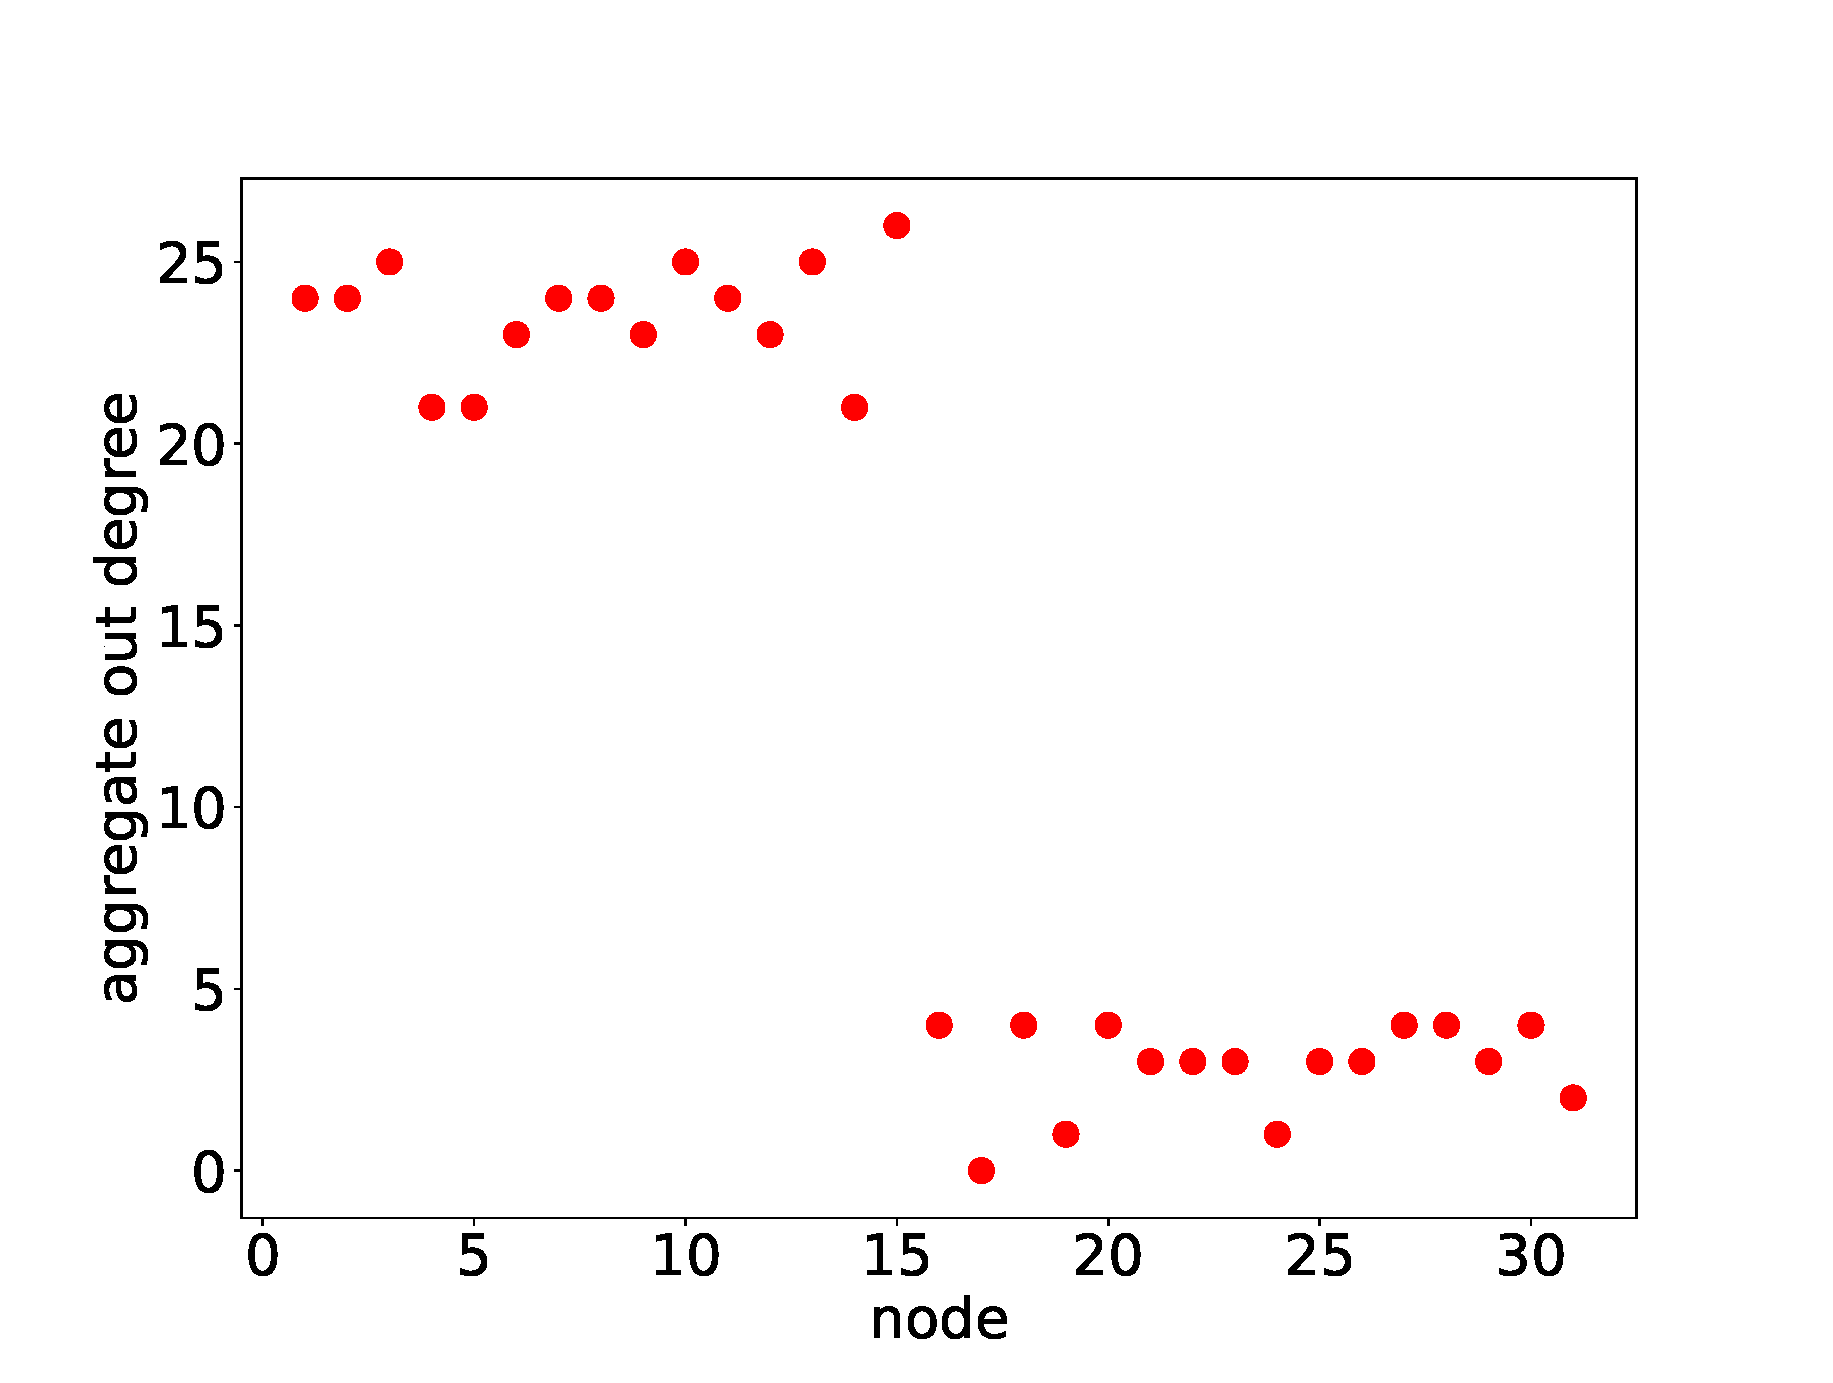
\includegraphics[width=\textwidth]{exp1_agg_out_degree}
         \caption{Aggregate out degree for each node}
         \label{fig:bt4}
     \end{subfigure}
        \caption{Results from the dynamic network in figure \ref{fig:exp1}.}
        \label{fig:fourbt}
\end{figure}

\newpage
Second synthetic experiment

\begin{figure}[h]\centering
    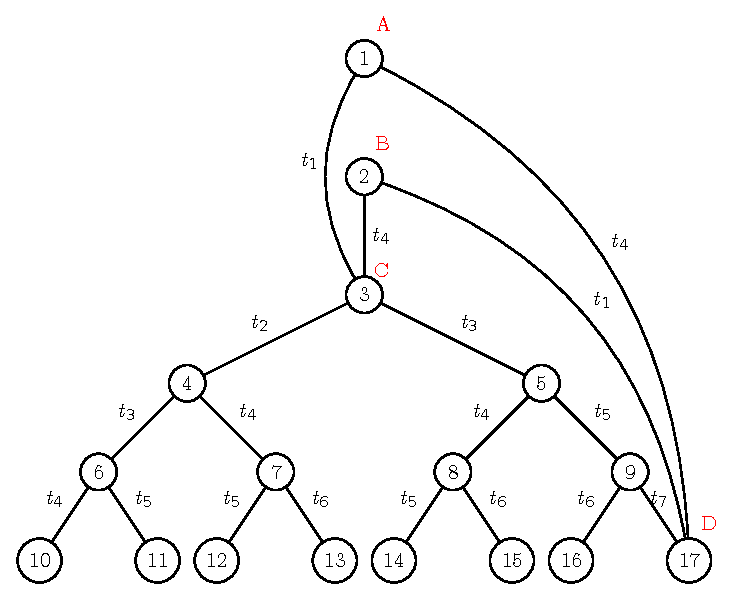
\includegraphics[width=.65\textwidth]{experiment2}
    \caption{Network structure for the second synthetic experiment. Links of A(t) are active over non-overlapping time intervals such that $t_i\coloneqq[(i − 1)\tau , (i − 1 + 0.9)\tau )$, for $i=0, 1, \dots , 7$, and $\tau =0.1$, repeated periodically over five cycles.}
    \label{fig:exp2}
    \bigskip
\end{figure}

\begin{figure}
     \centering
     \begin{subfigure}[b]{0.49\textwidth}
         \centering
         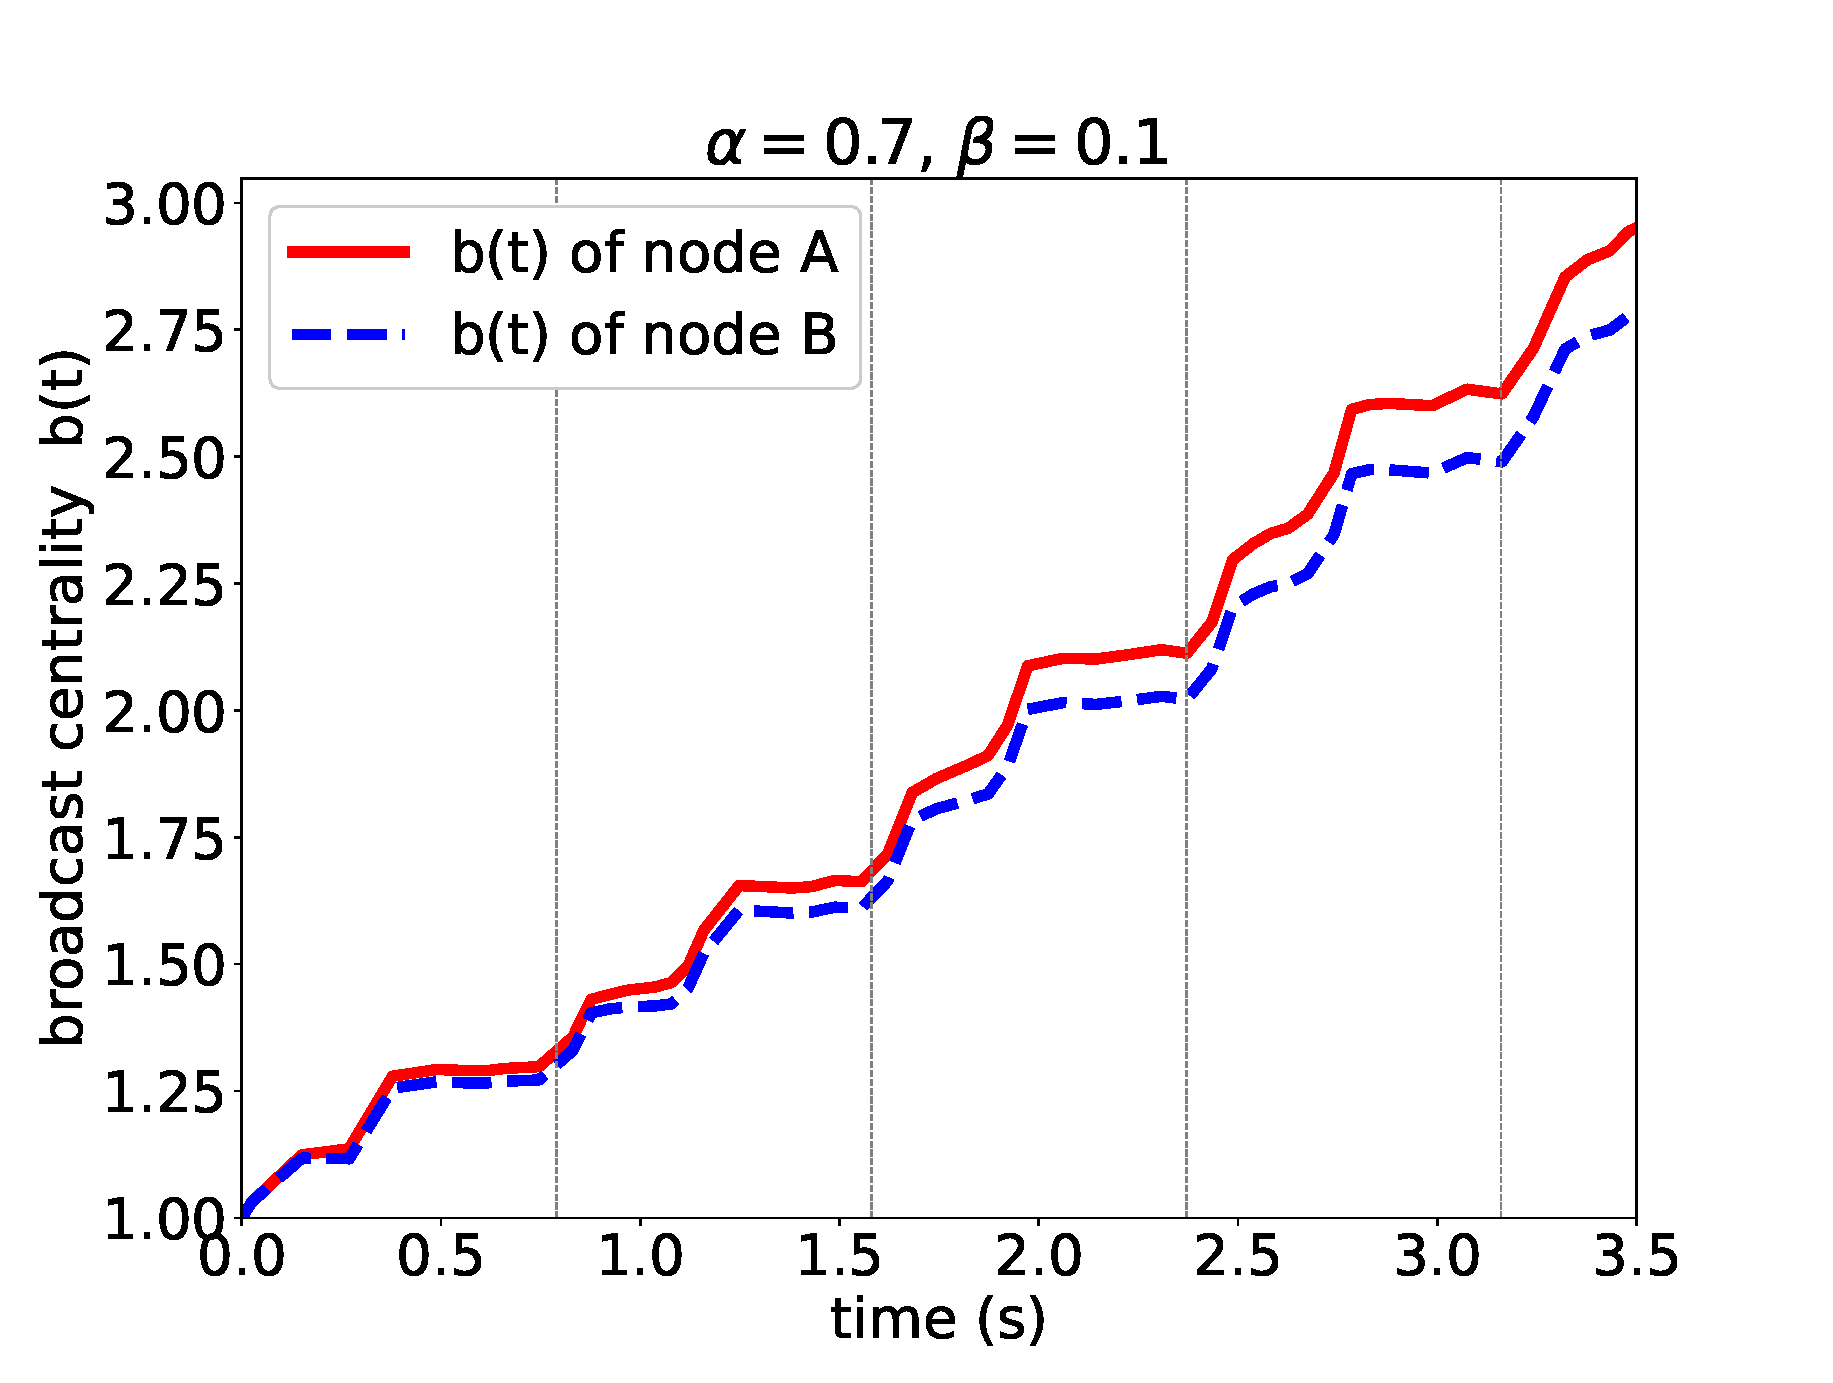
\includegraphics[width=\textwidth]{exp2b_btA_vs_btB}
         \caption{broadcast for $\alpha = 0.7 ,~\beta = 0.1$}
         \label{fig:bt5}
     \end{subfigure}
     \hfill
     \begin{subfigure}[b]{0.49\textwidth}
         \centering
         \includegraphics[width=\textwidth]{exp2a_btA_vs_btB}
         \caption{broadcast for $\alpha = 0.9 ,~\beta = 0.1$}
         \label{fig:bt6}
     \end{subfigure}
     \caption{Dynamic broadcast centrality over time for node A (solid) and node B (dashed) in the network of figure \ref{fig:exp2}.}
     \label{fig:twobt}
\end{figure}

\newpage
\section{Voice call experiment}
\label{sec:voicecall}

